\chapter{Конструкторский раздел}

В данном разделе проводиться требования к разработке метода для устранения размытия на изображениях, программное обеспечение для его применения далее рассмотривается основнные моменты разработки метода и программного обеспечения для устранения размытия на изображениях.

\section{Требования к Разработке Метода}

При разработке метода для устранения эффекта размытия на изображениях с использованием нейронных сетей необходимо учесть следующие требования:

\begin{enumerate}
    \item Ввод изображений:
    \begin{itemize}
        \item Метод должен поддерживать загрузку изображений в различных форматах для обеспечения удобства пользователя.
    \end{itemize}

    \item Устранение размытия с сохранением деталей:
    \begin{itemize}
        \item Основная задача метода - эффективное устранение размытия, сохраняя при этом детали и качество изображения.
        \item Метод должен восстанавливать четкость и резкость краев объектов на изображении.
    \end{itemize}

    \item Представление результатов и оценка качества:
    \begin{itemize}
        \item Результаты работы метода должны быть визуально представлены пользователю для оценки эффективности.
        \item Проведение оценки качества работы метода с использованием объективных метрик, таких как PSNR и SSIM.
    \end{itemize}

    \item Применение нейронных сетей для устранения размытия:
    \begin{itemize}
        \item Метод должен использовать нейронные сети для эффективного обучения на больших объемах данных и выявления сложных закономерностей в изображениях.
        \item Нейронные сети должны быть специально адаптированы для задачи устранения размытия.
    \end{itemize}
\end{enumerate}

\section{Требования к программному Обеспечению}

При разработке программного комплекса, взаимодействующего с методом устранения размытия на изображениях, необходимо учесть следующие требования:

\begin{enumerate}
    \item Загрузка изображений через интерфейс:
    \begin{itemize}
        \item Пользователь должен иметь возможность легко загружать изображения в программу через простой интерфейс.
    \end{itemize}

    \item Просмотр результатов работы метода и сравнение с исходным изображением:
    \begin{itemize}
        \item После применения метода устранения размытия, пользователь должен иметь возможность просмотреть результат на экране.
    \end{itemize}

    \item Поддержка сравнения с оригинальным изображением:
    \begin{itemize}
        \item Программный комплекс должен предоставлять возможность прямого сравнения очищенного изображения с оригинальным для более детальной оценки результатов.
    \end{itemize}
\end{enumerate}

На рисунке (\ref{fig:use-case}) представлено, диаграмма вариантов использования программного обеспечения: 
\begin{figure}[H]
	\centering
	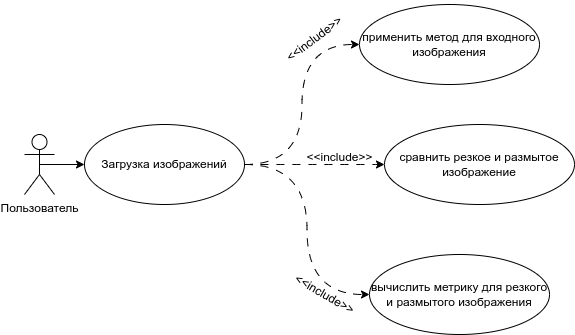
\includegraphics[width=0.5\linewidth]{assets/use-case-diagram.png}
	\caption{Диаграмма вариантов использования программного обеспечения}
	\label{fig:use-case}
\end{figure}


\section{Требования к корпусы данных}

Корпусы данных в работе метода играет главную роль, так как будщие работы метода будет относиться к ними,  требования к корпусам данных для обучения метода устранения размытия на изображениях с использованием нейронных сетей могут быть следующими:

\begin{enumerate}
    \item Разнообразие изображений:
    \begin{itemize}
        \item Корпус данных должен включать в себя широкий спектр изображений различных типов и содержания, чтобы метод был адаптирован к различным сценариям использования.
    \end{itemize}

    \item Разнообразие уровней размытия:
    \begin{itemize}
        \item Данные должны представлять изображения с различными уровнями размытия, чтобы обученная модель была способна эффективно устранять размытие в различных условиях.
    \end{itemize}

    \item Размер и разрешение изображений:
    \begin{itemize}
        \item Изображения должны иметь различные размеры и разрешения, чтобы модель была способна обрабатывать изображения различных форматов и разрешений.
    \end{itemize}

    \item Разделение на обучающую, валидационную и тестовую выборки:
    \begin{itemize}
        \item Корпус данных должен быть разделен на независимые обучающую, валидационную и тестовую выборки для эффективного обучения, валидации и оценки модели.
    \end{itemize}
\end{enumerate}

\section{Проектирование метода устранение размытия на изображениях}

Судя по перечисленным требованиям по устранению размытия на изображениях и проведенных сравнение по критерям в таблице (\ref{tab:comparison}), подходящим методом для этой цели является MPRNet. Метод хорошо справляется с задачами восстановления изображений и его следует спроектировать таким образом, чтобы он мог эффективно решать задачу устранения размытия на изображениях.

На рисунке (\ref{fig:mprnet-flowchart}) представлено, схема работы разработанного метода: 
\begin{figure}[H]
	\centering
	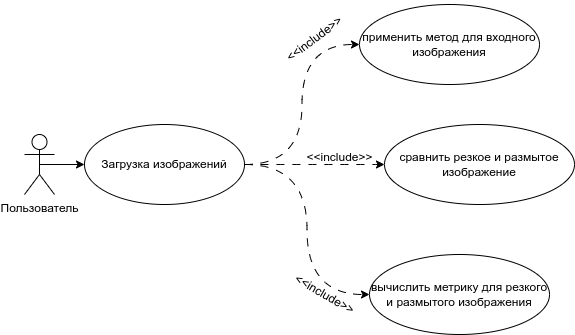
\includegraphics[width=0.5\linewidth]{assets/use-case-diagram.png}
	\caption{Схема работы MPRNet}
	\label{fig:mprnet-flowchart}
\end{figure}

Реализация сети многоступенчатого прогрессивного восстановления изображений (MPRNet) \cite{zamir2021multi} состоит из трех этапов для постепенного восстановления изображений. Первые два этапа имеют модель кодер-декодер, основанную на стандартной U-Net \cite{unet2015}, для получения полной контекстной информации входного изображения. На последнем этапе подсеть исходного разрешения (ORSNet) работает с исходным разрешением изображения, генерируя пространственно точные выходные данные для пиксельного соответствия между входными и выходными изображениями, перед тем как подаем в сеть изображение, так как изображение  если входное изображение не делится на 8 патчей, прежде чем подать его на вход нейронной сети, мы должны поработать с изображением и дополнить его пикселями, подробно рассмотрим алгоритмическую реализацию сети.



\subsection{Модель кодер-декодер}

